\section{三维旋转}
\label{sec:lie-rotations}

三维朝向有三个自由度，却没有一种记录方式能同时做到“恰好三个实数、处处无奇异、每个朝向只有一个记录”。本节围绕同一个旋转比较几种表示：旋转矩阵直接作用在向量上，轴角把旋转写成Lie代数元素的指数，Euler角依次绕坐标轴转动，单位四元数用四个数和一个长度约束完成复合。

对每种表示，我们分别说明它的计算规则、哪些参数给出同一个旋转，以及在哪里不能作为局部坐标。下面固定约定：旋转主动地作用在列向量上，$\bm x'=\bm R\bm x$；先作用$\bm R_1$、后作用$\bm R_2$的复合是$\bm R_2\bm R_1$。不同文献对主动与被动、左乘与右乘的约定不同，同一个公式在两种约定下的含义可能相反。关于四元数的约定比较可查阅\scite{math-sola2017quaternion}。

先说明“全局三参数坐标”为什么不可能。类比是地图：地球表面无法用一张没有裂缝的平面地图覆盖，$\mathrm{SO}(3)$也无法用$\mathbb R^3$中的一张坐标图覆盖。

\begin{theorem}[三维旋转群没有单张坐标图]
\label{thm:lie-so3-no-global-chart}
$\mathrm{SO}(3)$是紧的三维流形，不存在从$\mathrm{SO}(3)$到$\mathbb R^3$中开集的同胚。
\end{theorem}

\begin{proof}
$\mathrm{SO}(3)$是连续映射$\bm R\mapsto(\bm R^\top\bm R,\det\bm R)$下一点的原像，因而在$\mathbb R^{3\times3}$中是闭集。它也有界，因为
\[
\lVert\bm R\rVert_{\mathrm F}^2=\operatorname{tr}(\bm R^\top\bm R)=3.
\]
所以$\mathrm{SO}(3)$是紧集。

假设$\varphi:\mathrm{SO}(3)\to U$是到开集$U\subseteq\mathbb R^3$的同胚。连续映射把紧集映成紧集，所以$U$是紧集，从而在$\mathbb R^3$中是闭集。

于是$U$非空且既开又闭。由$\mathbb R^3$连通，得到$U=\mathbb R^3$，但$\mathbb R^3$不是紧集，矛盾。
\end{proof}

所以任何三参数表示都只能在局部充当坐标，必然在某处出现冗余或奇异；单位四元数用四个参数换取处处正常的局部性质，代价是每个旋转有两个记录。

\subsection{旋转矩阵与轴角}
\label{sec:lie-rotation-axis-angle}

旋转矩阵是旋转最直接的记录，轴角则是它在Lie代数中的坐标。本小节由矩阵条件出发，用矩阵指数连接二者，再说明轴角及另一种常见的三角度记录各在哪里失效。

\paragraph{旋转矩阵}
三维旋转保持长度与夹角，所以保持内积：$(\bm R\bm x)^\top(\bm R\bm y)=\bm x^\top\bm y$对所有$\bm x,\bm y$成立，等价于$\bm R^\top\bm R=\bm I$。正交矩阵的行列式为$\pm1$，其中$\operatorname{diag}(1,1,-1)$关于一个平面作镜面反射，把右手坐标系变成左手坐标系。要求保持定向，就是要求$\det\bm R=1$。于是三维旋转组成
\[
\mathrm{SO}(3)=\{\bm R\in\mathbb R^{3\times3}:\bm R^\top\bm R=\bm I,\ \det\bm R=1\},
\]
称为\term{三维旋转群}（three-dimensional rotation group）。由定理~\ref{thm:lie-orthogonal-group-manifold}，它是三维流形，$\bm R$处的切向量是$\bm R[\bm\omega]_\times$，其中$[\bm\omega]_\times$由式~\eqref{eq:lie-hat-map}给出。

\paragraph{Rodrigues公式}
旋转的Lie代数由角速度向量$\bm\omega$记录。写$\bm\omega=\theta\bm u$，其中$\lVert\bm u\rVert_2=1$、$\theta\geq0$，就可以按轴与角计算指数。关键是$[\bm u]_\times$的各次幂只有两种形状。由二重叉积公式，
\[
[\bm u]_\times^2\bm x=\bm u\times(\bm u\times\bm x)=\bm u(\bm u^\top\bm x)-\bm x,
\]
也就是
\begin{equation}
 [\bm u]_\times^2=\bm u\bm u^\top-\bm I.
 \label{eq:lie-hat-square}
\end{equation}

再乘一次$[\bm u]_\times$，由$\bm u\times\bm u=\bm0$得到$[\bm u]_\times^3=-[\bm u]_\times$。所以奇次幂都是$\pm[\bm u]_\times$，正的偶次幂都是$\pm[\bm u]_\times^2$，指数级数可以按奇偶项汇总。

\begin{theorem}[Rodrigues公式]
\label{thm:lie-rodrigues}
对单位向量$\bm u\in\mathbb R^3$与$\theta\in\mathbb R$，
\begin{equation}
 \exp(\theta[\bm u]_\times)=\bm I+\sin\theta\,[\bm u]_\times+(1-\cos\theta)[\bm u]_\times^2.
 \label{eq:lie-rodrigues}
\end{equation}
它保持$\bm u$不动，并把与$\bm u$正交的向量$\bm x$变成$\cos\theta\,\bm x+\sin\theta\,\bm u\times\bm x$。
\end{theorem}

\begin{proof}
对$k\geq1$，有$[\bm u]_\times^{2k+1}=(-1)^k[\bm u]_\times$，$[\bm u]_\times^{2k}=(-1)^{k-1}[\bm u]_\times^2$。把式~\eqref{eq:lie-matrix-exponential}按奇偶项汇总，得到
\[
\exp(\theta[\bm u]_\times)=\bm I
+\Bigl(\theta-\frac{\theta^3}{3!}+\cdots\Bigr)[\bm u]_\times
+\Bigl(\frac{\theta^2}{2!}-\frac{\theta^4}{4!}+\cdots\Bigr)[\bm u]_\times^2,
\]
两个括号分别是$\sin\theta$与$1-\cos\theta$，这就是式~\eqref{eq:lie-rodrigues}。

又$[\bm u]_\times\bm u=\bm0$，代入式~\eqref{eq:lie-rodrigues}得$\bm u$不动。若$\bm u^\top\bm x=0$，由式~\eqref{eq:lie-hat-square}得$[\bm u]_\times^2\bm x=-\bm x$，代入式~\eqref{eq:lie-rodrigues}，得到
\[
\exp(\theta[\bm u]_\times)\bm x
=\bm x+\sin\theta\,\bm u\times\bm x-(1-\cos\theta)\bm x
=\cos\theta\,\bm x+\sin\theta\,\bm u\times\bm x.\qedhere
\]
\end{proof}

这个公式称为\term{Rodrigues公式}（Rodrigues' formula）。把任一向量分解为沿轴的分量和垂直于轴的分量，沿轴的部分不动，垂直的部分在垂直于轴的平面内转动角$\theta$，这就是式~\eqref{eq:lie-rodrigues}的几何含义。由上一节，反对称矩阵的指数必在$\mathrm{SO}(3)$中，所以式~\eqref{eq:lie-rodrigues}总给出合法的旋转：绕轴$\bm u$按右手方向转角$\theta$。

手算一个例子。取$\bm u=(1,1,1)^\top/\sqrt3$，$\theta=2\pi/3$，于是
\[
\sin\theta=\frac{\sqrt3}2,\qquad\cos\theta=-\frac12 .
\]
把$\bm x=\bm e_1$分解为沿轴和垂直于轴的两部分，得到
\[
\bm x_\parallel=(\bm u^\top\bm e_1)\bm u=\tfrac13(1,1,1)^\top,\qquad
\bm x_\perp=\bm e_1-\bm x_\parallel=\tfrac13(2,-1,-1)^\top.
\]

计算垂直部分的叉积，得到
\[
\bm u\times\bm x_\perp=\frac{1}{\sqrt3}(0,1,-1)^\top .
\]
代入定理的第二个结论，垂直部分转动后是
\[
\cos\theta\,\bm x_\perp+\sin\theta\,\bm u\times\bm x_\perp
=-\tfrac16(2,-1,-1)^\top+\tfrac12(0,1,-1)^\top
=\tfrac13(-1,2,-1)^\top .
\]

加回沿轴部分$\frac13(1,1,1)^\top$，结果是$(0,1,0)^\top=\bm e_2$。对$\bm e_2,\bm e_3$同样计算，整个矩阵是把坐标轴循环轮换的矩阵
\[
\bm R=\begin{bmatrix}0&0&1\\1&0&0\\0&1&0\end{bmatrix}.
\]
图~\ref{fig:lie-rodrigues-decomposition}画出了这次分解。

\begin{BookInlineFigure}
  \centering
  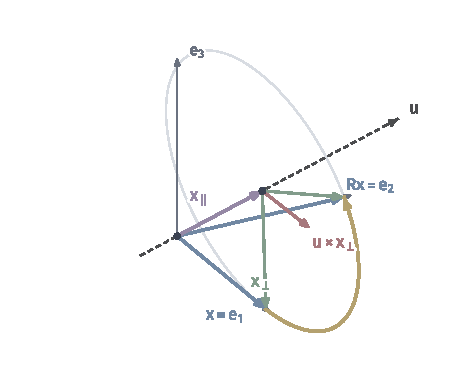
\includegraphics[width=80mm]{figures/04-spaces-measures-and-geometry/04-manifolds/matplotlib/lie-rodrigues-decomposition/figure.pdf}
  \caption{Rodrigues公式的分解。旋转轴$\bm u=(1,1,1)^\top/\sqrt3$，转角$2\pi/3$，$\bm x=\bm e_1$。紫色是沿轴分量$\bm x_\parallel$，保持不动；绿色是垂直分量$\bm x_\perp$，在灰色圆所在的平面内转动，转完后的绿色向量指向$\bm R\bm x$的末端；红色是$\bm u\times\bm x_\perp$的方向（长度按比例缩短）；黄色弧是端点走过的路径，终点是$\bm R\bm x=\bm e_2$。}
  \label{fig:lie-rodrigues-decomposition}
\end{BookInlineFigure}

\paragraph{每个旋转都有轴与角}
反过来，每个三维旋转都能写成式~\eqref{eq:lie-rodrigues}的形式，从而$\exp:\mathfrak{so}(3)\to\mathrm{SO}(3)$是满射。要证明这一点，先找出旋转的转轴，它是特征值$1$的特征向量，再看垂直于轴的平面。

\begin{theorem}[轴角表示]
\label{thm:lie-axis-angle}
对每个$\bm R\in\mathrm{SO}(3)$，存在单位向量$\bm u$与$\theta\in[0,\pi]$，使$\bm R=\exp(\theta[\bm u]_\times)$。并且
\begin{equation}
 \operatorname{tr}\bm R=1+2\cos\theta,\qquad \bm R-\bm R^\top=2\sin\theta\,[\bm u]_\times.
 \label{eq:lie-axis-angle-recovery}
\end{equation}
\end{theorem}

\begin{proof}
先找转轴。由$\bm R^\top\bm R=\bm I$与$\det\bm R=1$，得到
\[
\det(\bm R-\bm I)=\det\bigl(\bm R(\bm I-\bm R^\top)\bigr)
=\det(\bm I-\bm R^\top)=\det(\bm I-\bm R).
\]
三阶矩阵取负号使行列式变号，$\det(\bm I-\bm R)=-\det(\bm R-\bm I)$，于是$\det(\bm R-\bm I)=0$，存在单位向量$\bm u$使$\bm R\bm u=\bm u$。

再看与轴正交的平面。若$\bm x^\top\bm u=0$，则
\[
(\bm R\bm x)^\top\bm u=(\bm R\bm x)^\top(\bm R\bm u)=\bm x^\top\bm u=0,
\]
所以平面$\bm u^\perp$被$\bm R$映到自身。

取$\bm u^\perp$中的单位向量$\bm v$，令$\bm w=\bm u\times\bm v$，则$(\bm v,\bm w,\bm u)$是右手标准正交基。在这组基下$\bm R$的矩阵是分块对角的，左上二阶块正交，且行列式等于$\det\bm R=1$。由第~\ref{sec:lie-group-subgroup}节对$\mathrm{SO}(2)$的刻画，它等于某个$\bm R(\theta)$，$\theta\in[0,2\pi)$，即$\bm R\bm v=\cos\theta\,\bm v+\sin\theta\,\bm w$。

若$\theta\in(\pi,2\pi)$，把$\bm u$换成$-\bm u$、$\theta$换成$2\pi-\theta$，于是可取$\theta\in[0,\pi]$。这与定理~\ref{thm:lie-rodrigues}描述的作用在一组基上一致，所以二者相等。

最后，对式~\eqref{eq:lie-rodrigues}取迹。反对称矩阵的迹为零，并由式~\eqref{eq:lie-hat-square}，
\[
\operatorname{tr}[\bm u]_\times^2=\operatorname{tr}(\bm u\bm u^\top)-3=-2,
\]
于是
\[
\operatorname{tr}\bm R=3-2(1-\cos\theta)=1+2\cos\theta.
\]
减去转置时对称部分抵消，反对称部分加倍，得到第二式。
\end{proof}

这给出\term{轴角表示}（axis-angle representation），常把它合成一个向量$\bm\omega=\theta\bm u$，称为旋转向量。用式~\eqref{eq:lie-axis-angle-recovery}反算上面的循环轮换矩阵。它的迹为$0$，所以$\cos\theta=-\frac12$，$\theta=2\pi/3$。反对称部分给出
\[
\bm R-\bm R^\top=\begin{bmatrix}0&-1&1\\1&0&-1\\-1&1&0\end{bmatrix}
=2\sin\theta\,[\bm u]_\times,
\]
对照式~\eqref{eq:lie-hat-map}读出$\bm u\propto(1,1,1)^\top$，再由$2\sin\theta=\sqrt3$得到$\bm u=(1,1,1)^\top/\sqrt3$，回到了原来的轴和角。

\paragraph{冗余与特殊角度}
轴角表示有三类冗余。$(\bm u,\theta)$与$(-\bm u,-\theta)$给出同一旋转，$\theta$与$\theta+2\pi$也给出同一旋转，所以把$\theta$限制在$[0,\pi]$。在这个范围内，$0<\theta<\pi$时$\sin\theta>0$，式~\eqref{eq:lie-axis-angle-recovery}唯一地恢复$\theta$与$\bm u$。

剩下两个角度需要单独说明。$\theta=0$时$\bm R=\bm I$，任何轴都可以。$\theta=\pi$时$\bm R-\bm R^\top=\bm0$，轴$\bm u$与$-\bm u$给出同一旋转：绕一个轴转半圈，与绕相反的轴转半圈结果相同。

用旋转向量描述，映射$\bm\omega\mapsto\exp([\bm\omega]_\times)$把闭球$\{\lVert\bm\omega\rVert_2\leq\pi\}$映满$\mathrm{SO}(3)$；在开球$\lVert\bm\omega\rVert_2<\pi$内是单射，边界球面上互为相反数的两点给出同一个旋转。所以$\mathrm{SO}(3)$可以想象成一个实心球，球面上相对的点被粘合。

图~\ref{fig:lie-so3-ball}用这个模型画出绕$\bm e_3$的旋转：$\theta$从$0$增大到$\pi$时，$\bm\omega$沿半径走到$\pi\bm e_3$；继续增大，它从球面相对的一点$-\pi\bm e_3$重新进入，回到中心。这条路径在$\mathrm{SO}(3)$中是连续的闭合路径，并没有跳跃。

\begin{BookInlineFigure}
  \centering
  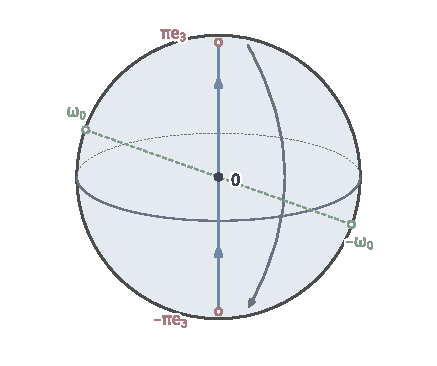
\includegraphics[width=74mm]{figures/04-spaces-measures-and-geometry/04-manifolds/matplotlib/lie-so3-ball/figure.pdf}
  \caption{$\mathrm{SO}(3)$的实心球模型。每个旋转向量$\bm\omega$的长度是转角，方向是转轴，闭球半径为$\pi$。边界上相对的两点（红圈$\pm\pi\bm e_3$，绿圈$\pm\bm\omega_0$）表示同一个旋转。蓝线是绕$\bm e_3$转一周的路径，走到$\pi\bm e_3$后，灰箭头表示它在$-\pi\bm e_3$处接着走，整条路径在$\mathrm{SO}(3)$中连续。}
  \label{fig:lie-so3-ball}
\end{BookInlineFigure}

在开球内，逆映射由式~\eqref{eq:lie-axis-angle-recovery}给出：
\[
\theta=\arccos\frac{\operatorname{tr}\bm R-1}{2},\qquad
[\bm\omega]_\times=\frac{\theta}{2\sin\theta}(\bm R-\bm R^\top),
\]
其中$\theta=0$处按极限$\theta/\sin\theta\to1$理解。所以旋转向量是$\mathrm{SO}(3)$去掉全部半圈旋转之后的局部坐标，与定理~\ref{thm:lie-so3-no-global-chart}一致：它不能延伸成全局坐标。

\paragraph{局部更新}
在一个已知旋转$\bm R$附近，常用$\bm R\exp([\bm\delta]_\times)$表示扰动后的旋转，其中$\bm\delta\in\mathbb R^3$很小。这是把单位元附近的指数坐标左平移到$\bm R$附近，参数$\bm\delta$在$\lVert\bm\delta\rVert_2<\pi$内与旋转一一对应。

一阶近似$\bm R+\bm R[\bm\delta]_\times$只是切空间中的一步，一般已不是正交矩阵；用指数代替它，结果严格留在$\mathrm{SO}(3)$中，这正是图~\ref{fig:lie-exp-limit}中折线与圆弧的区别。右乘$\exp([\bm\delta]_\times)$在物体自身的坐标系中扰动，左乘$\exp([\bm\delta]_\times)\bm R$则在固定的外部坐标系中扰动，二者一般不同，使用时须说明。

\paragraph{Euler角与万向节锁}
另一种常见的三参数记录是依次绕坐标轴旋转。记$\bm R_x,\bm R_y,\bm R_z$为绕三个坐标轴的旋转，取
\begin{equation}
 \bm R(\alpha,\beta,\gamma)=\bm R_z(\alpha)\bm R_y(\beta)\bm R_x(\gamma),
 \label{eq:lie-euler-angles}
\end{equation}
三个角称为一组\term{Euler角}（Euler angles）。它便于解释，却在特殊角度失去局部坐标的作用，原因在于三个参数对应的瞬时转轴可能共线。

把式~\eqref{eq:lie-euler-angles}分别对三个角求导，再右乘$\bm R^\top$，得到每个参数产生的角速度方向。用$\bm R_z(\alpha)$与$\bm R_y(\beta)$共轭后，三个方向是
\[
\bm a_\alpha=\bm e_3,\qquad
\bm a_\beta=\bm R_z(\alpha)\bm e_2,\qquad
\bm a_\gamma=\bm R_z(\alpha)\bm R_y(\beta)\bm e_1 .
\]
以$\bm a_\gamma$为例，把$\bm R_x$的导数写成$\bm R_x[\bm e_1]_\times$（绕$\bm e_1$转动的方向），再把两侧的转动并进叉积，得到
\[
\partial_\gamma\bm R\,\bm R^\top
=\bm R_z\bm R_y[\bm e_1]_\times\bm R_y^\top\bm R_z^\top
=[\bm R_z\bm R_y\bm e_1]_\times .
\]

这三个方向的线性无关性决定了参数化是否满秩。由
\[
\bm R_y(\beta)\bm e_1=(\cos\beta,0,-\sin\beta)^\top,
\]
并把三个向量都乘以$\bm R_z(\alpha)^\top$（不改变行列式），得到
\[
\det[\bm a_\alpha,\bm a_\beta,\bm a_\gamma]
=\det\begin{bmatrix}0&0&\cos\beta\\0&1&0\\1&0&-\sin\beta\end{bmatrix}
=-\cos\beta .
\]
当$\beta=\pm\pi/2$时行列式为零，参数到旋转的微分秩降为$2$。

\begin{BookInlineFigure}
  \centering
  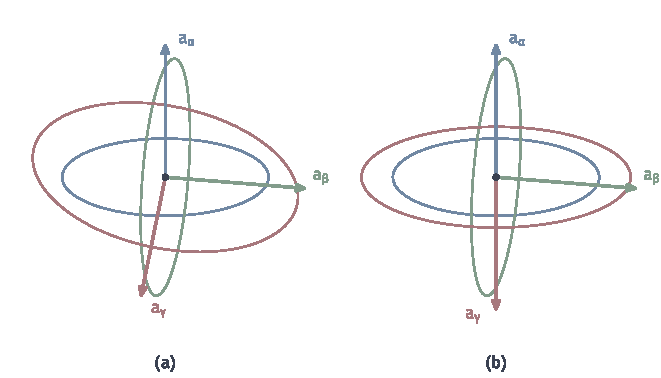
\includegraphics[width=112mm]{figures/04-spaces-measures-and-geometry/04-manifolds/matplotlib/lie-gimbal-lock/figure.pdf}
  \caption{Euler角的三个瞬时转轴。蓝、绿、红箭头分别是$\alpha,\beta,\gamma$对应的转轴$\bm a_\alpha,\bm a_\beta,\bm a_\gamma$，同色圆环垂直于该轴（这里$\alpha=20^\circ$）。(a)$\beta=35^\circ$，三根轴线性无关，任何方向的小转动都能实现。(b)$\beta=90^\circ$，$\bm a_\gamma=-\bm e_3$与$\bm a_\alpha$共线，两个圆环重合在同一平面内，只剩两个独立的转动方向。}
  \label{fig:lie-gimbal-lock}
\end{BookInlineFigure}

直接代入也能看到这一点。由$\bm R_y(\pi/2)\bm e_1=-\bm e_3$，绕$\bm e_1$的旋转经$\bm R_y(\pi/2)$共轭后变为绕$-\bm e_3$的旋转，即
\[
\bm R_y(\tfrac\pi2)\bm R_x(\gamma)=\bm R_z(-\gamma)\bm R_y(\tfrac\pi2).
\]
于是
\[
\bm R(\alpha,\tfrac\pi2,\gamma)=\bm R_z(\alpha-\gamma)\bm R_y(\tfrac\pi2).
\]
结果只依赖$\alpha-\gamma$：同时把$\alpha,\gamma$加上同一个数，旋转不变。这称为\term{万向节锁}（gimbal lock），图~\ref{fig:lie-gimbal-lock}(b)中蓝、红两根轴共线正是它的几何原因。

万向节锁是坐标的奇异，不是旋转本身的退化。$\bm R(\alpha,\pi/2,\gamma)$仍是合法的旋转，$\mathrm{SO}(3)$在它附近仍是三维流形；只是这一组角在该处不能作为坐标，附近的小转动也可能要求角度大幅跳动。换一种轴的次序或改用旋转向量，就能在这里重新得到正常的局部坐标。

\subsection{单位四元数}
\label{sec:lie-unit-quaternions}

旋转矩阵用九个数，轴角在半圈处与恒等处需要特别处理。单位四元数用四个数和一个单位长度约束记录旋转，复合只需一次乘法，并且在每一点附近都给出正常的局部坐标，代价是每个旋转恰有两个记录。

\paragraph{四元数及其运算}
把\term{四元数}（quaternion）写成标量部与三维向量部组成的对$q=(s,\bm u)$，其中$s\in\mathbb R$、$\bm u\in\mathbb R^3$。加法与数乘按$\mathbb R^4$进行，乘法规定为
\begin{equation}
 (s,\bm u)(t,\bm v)=(st-\bm u^\top\bm v,\ s\bm v+t\bm u+\bm u\times\bm v).
 \label{eq:lie-quaternion-product}
\end{equation}
类比复数：标量部相当于实部，向量部相当于“虚部”，只是虚部有三个方向，它们之间的乘法由叉积描述。

因为含有叉积，乘法一般不交换：$(0,\bm e_1)(0,\bm e_2)=(0,\bm e_3)$，而$(0,\bm e_2)(0,\bm e_1)=(0,-\bm e_3)$。$(1,\bm0)$是乘法单位元。乘法满足结合律，把三重乘积按式~\eqref{eq:lie-quaternion-product}展开，用二重叉积公式整理即可验证，这里略去这段机械的展开。

共轭定义为$q^*=(s,-\bm u)$，范数定义为$\lvert q\rvert=\sqrt{s^2+\lVert\bm u\rVert_2^2}$，即$\mathbb R^4$中的欧氏长度。由式~\eqref{eq:lie-quaternion-product}，
\[
qq^*=\bigl(s^2+\bm u^\top\bm u,\ -s\bm u+s\bm u-\bm u\times\bm u\bigr)
=(\lvert q\rvert^2,\bm0),
\]
同理$q^*q=(\lvert q\rvert^2,\bm0)$。直接展开还可验证$(pq)^*=q^*p^*$。

下面的引理说明范数与乘法相容，这是四元数能表示旋转的基础。

\begin{lemma}[范数的乘法性]
\label{lem:lie-quaternion-norm}
对四元数$p,q$，$\lvert pq\rvert=\lvert p\rvert\,\lvert q\rvert$。因此$\lvert q\rvert=1$的\term{单位四元数}（unit quaternion）在乘法下构成群，$q^{-1}=q^*$；作为集合，它就是$\mathbb R^4$中的单位球面$S^3$。
\end{lemma}

\begin{proof}
设$p=(s,\bm u)$、$q=(t,\bm v)$。向量部$s\bm v+t\bm u+\bm u\times\bm v$中，$\bm u\times\bm v$与$\bm u,\bm v$都正交，所以
\[
\lvert pq\rvert^2=(st-\bm u^\top\bm v)^2+\lVert s\bm v+t\bm u\rVert_2^2+\lVert\bm u\times\bm v\rVert_2^2.
\]
展开平方后，交叉项$-2st\,\bm u^\top\bm v$与$+2st\,\bm u^\top\bm v$相消，剩下
\[
s^2t^2+s^2\lVert\bm v\rVert_2^2+t^2\lVert\bm u\rVert_2^2+(\bm u^\top\bm v)^2+\lVert\bm u\times\bm v\rVert_2^2.
\]
由Lagrange恒等式
\[
(\bm u^\top\bm v)^2+\lVert\bm u\times\bm v\rVert_2^2=\lVert\bm u\rVert_2^2\lVert\bm v\rVert_2^2,
\]
上式等于
\[
(s^2+\lVert\bm u\rVert_2^2)(t^2+\lVert\bm v\rVert_2^2).
\]
于是单位四元数的乘积仍是单位四元数，$qq^*=(1,\bm0)$给出逆元，结合律继承自全体四元数。
\end{proof}

\paragraph{用共轭作用表示旋转}
把向量$\bm x$嵌入为向量部，即纯四元数$(0,\bm x)$。对单位四元数$q=(s,\bm u)$，分两步计算$q(0,\bm x)q^*$。先由式~\eqref{eq:lie-quaternion-product}左乘，得到
\[
q(0,\bm x)=(-\bm u^\top\bm x,\ s\bm x+\bm u\times\bm x).
\]

再右乘$q^*=(s,-\bm u)$。标量部是
\[
(-\bm u^\top\bm x)s+(s\bm x+\bm u\times\bm x)^\top\bm u=0,
\]
这是因为$\bm u\times\bm x$与$\bm u$正交。向量部用二重叉积公式
\[
(\bm u\times\bm x)\times\bm u=\lVert\bm u\rVert_2^2\bm x-(\bm u^\top\bm x)\bm u
\]
整理，得到
\begin{equation}
 \begin{gathered}
 q(0,\bm x)q^*=(0,\bm R(q)\bm x),\\
 \bm R(q)\bm x=(s^2-\lVert\bm u\rVert_2^2)\bm x+2\bm u(\bm u^\top\bm x)+2s\,\bm u\times\bm x.
 \end{gathered}
 \label{eq:lie-quaternion-rotation}
\end{equation}

取$q=(\cos\frac\theta2,\ \sin\frac\theta2\,\bm a)$，其中$\lVert\bm a\rVert_2=1$。由半角公式，
\[
s^2-\lVert\bm u\rVert_2^2=\cos\theta,\qquad
2\bm u\bm u^\top=(1-\cos\theta)\bm a\bm a^\top,\qquad
2s\bm u=\sin\theta\,\bm a.
\]
代入式~\eqref{eq:lie-quaternion-rotation}，再用式~\eqref{eq:lie-hat-square}，得到
\[
\begin{aligned}
\bm R(q)
&=\cos\theta\,\bm I+(1-\cos\theta)\bm a\bm a^\top+\sin\theta\,[\bm a]_\times\\
&=\bm I+\sin\theta\,[\bm a]_\times+(1-\cos\theta)[\bm a]_\times^2 .
\end{aligned}
\]
这正是Rodrigues公式~\eqref{eq:lie-rodrigues}：$q$表示绕$\bm a$转角$\theta$。半角来自$q$在两侧各乘一次，不是把物理转角减半。

\paragraph{复合与双覆盖}
手算两个旋转的复合。设$q_1=(\frac{\sqrt2}2,\ \frac{\sqrt2}2\bm e_3)$表示绕$\bm e_3$转$90^\circ$，$q_2=(\frac{\sqrt2}2,\ \frac{\sqrt2}2\bm e_1)$表示绕$\bm e_1$转$90^\circ$，先做$q_1$、再做$q_2$。由式~\eqref{eq:lie-quaternion-product}，
\[
q_2q_1=\Bigl(\tfrac12,\ \tfrac12\bm e_3+\tfrac12\bm e_1+\tfrac12\bm e_1\times\bm e_3\Bigr)
=\Bigl(\tfrac12,\ \tfrac12(1,-1,1)^\top\Bigr).
\]

读出半角：$\cos\frac\theta2=\frac12$，所以$\theta=2\pi/3$，转轴是$(1,-1,1)^\top/\sqrt3$。用式~\eqref{eq:lie-quaternion-rotation}计算$\bm e_1$的像，三项分别是$-\frac12\bm e_1$、$\frac12(1,-1,1)^\top$、$\frac12(0,1,1)^\top$，相加得到$\bm e_3$。

直接用矩阵核对，
\[
\bm R_x(\tfrac\pi2)\bm R_z(\tfrac\pi2)\bm e_1=\bm R_x(\tfrac\pi2)\bm e_2=\bm e_3 ,
\]
结果一致。复合用四元数只需一次乘法，读出轴和角也只需看四个数。

这个计算说明的是一般事实。由结合律与$(q_2q_1)^*=q_1^*q_2^*$，
\[
(q_2q_1)(0,\bm x)(q_2q_1)^*=q_2\bigl(q_1(0,\bm x)q_1^*\bigr)q_2^* ,
\]
即$\bm R(q_2q_1)=\bm R(q_2)\bm R(q_1)$。所以$q\mapsto\bm R(q)$是从单位四元数群到$\mathrm{SO}(3)$的群同态。由定理~\ref{thm:lie-axis-angle}，每个旋转都有轴与角，从而有形如上式的四元数，这个同态是满射。它的核由下面的定理确定。

\begin{theorem}[单位四元数的双覆盖]
\label{thm:lie-double-cover}
对单位四元数$q_1,q_2$，$\bm R(q_1)=\bm R(q_2)$当且仅当$q_2=\pm q_1$。
\end{theorem}

\begin{proof}
由定理~\ref{thm:lie-kernel-injective}，只需证明核为$\{(1,\bm0),(-1,\bm0)\}$。设$q=(s,\bm u)$是单位四元数，$\bm R(q)=\bm I$。

若$\bm u\neq\bm0$，取与$\bm u$正交的非零向量$\bm x$。由式~\eqref{eq:lie-quaternion-rotation}与$s^2+\lVert\bm u\rVert_2^2=1$，$\bm x=\bm R(q)\bm x$成为
\[
\bm x=(1-2\lVert\bm u\rVert_2^2)\bm x+2s\,\bm u\times\bm x,
\]
移项得到
\[
-2\lVert\bm u\rVert_2^2\bm x+2s\,\bm u\times\bm x=\bm0 .
\]
两项分别与$\bm x$平行、与$\bm x$正交，必须各为零，第一项非零，矛盾。

所以$\bm u=\bm0$，由单位长度得$s=\pm1$。反过来，$\pm(1,\bm0)$代入式~\eqref{eq:lie-quaternion-rotation}给出$\bm I$。
\end{proof}

这称为单位四元数对$\mathrm{SO}(3)$的\term{双覆盖}（double cover）：每个旋转恰有两个单位四元数，二者互为相反数。上面的$q_1$与$-q_1=(-\frac{\sqrt2}2,-\frac{\sqrt2}2\bm e_3)$表示同一个旋转，后者对应转角$\pi/2+2\pi$的半角。图~\ref{fig:lie-double-cover}把$S^3$限制到一条大圆上画出这个现象。

\begin{BookInlineFigure}
  \centering
  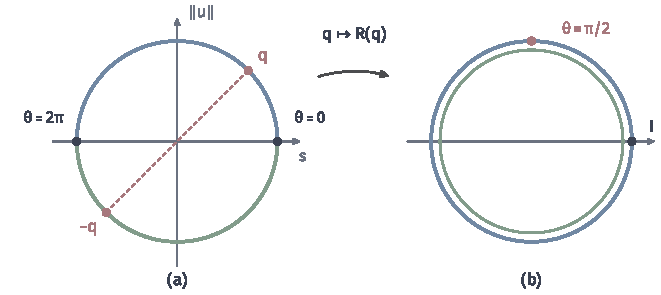
\includegraphics[width=112mm]{figures/04-spaces-measures-and-geometry/04-manifolds/matplotlib/lie-double-cover/figure.pdf}
  \caption{半角与双覆盖。固定转轴$\bm a$，单位四元数$(\cos\frac\theta2,\sin\frac\theta2\,\bm a)$在$S^3$中走出一条大圆。(a)这条大圆，横轴为标量部，纵轴为沿$\bm a$的向量部。$\theta$从$0$到$2\pi$时走过蓝色半圆，从$2\pi$到$4\pi$时走过绿色半圆，$q$与$-q$（红点）相对。(b)绕$\bm a$的旋转组成的圆，$\theta$走一周即回到$\bm I$，蓝、绿两个半圆分别映满整个圆，$q$与$-q$映到同一点。}
  \label{fig:lie-double-cover}
\end{BookInlineFigure}

双覆盖与坐标奇异是两回事。$q\mapsto\bm R(q)$在每一点都是局部微分同胚。在$q=(1,\bm0)$附近，
\[
\bm R(q)=\bm I+2[\bm u]_\times+O(\lVert\bm u\rVert_2^2),
\]
微分$\bm u\mapsto2[\bm u]_\times$是从切空间$T_{(1,\bm0)}S^3=\{(0,\bm u)\}$到$\mathfrak{so}(3)$的线性同构；在其他点用群乘法平移即得。

所以单位四元数在任何朝向附近都给出正常的局部坐标，不会出现Euler角那样的秩下降。$q$与$-q$之差也不是额外的物理自由度：$S^3$与$\mathrm{SO}(3)$都是三维，符号只是整体上的二选一。

\paragraph{计算中的注意事项}
按式~\eqref{eq:lie-quaternion-product}，两个四元数相乘需要$16$次实数乘法，两个三阶矩阵相乘需要$27$次。数值计算中多次相乘会使$\lvert q\rvert$逐渐偏离$1$；若$\lvert q\rvert\neq1$，$q(0,\bm x)q^*$会额外把$\bm x$放大$\lvert q\rvert^2$倍，不再是旋转，所以需要定期把$q$除以$\lvert q\rvert$。

比较两个四元数是否接近时，还要考虑符号：$q$与$-q$在$\mathbb R^4$中相距$2$，表示的却是同一个旋转。表~\ref{tab:lie-rotation-representations}汇总了本节比较的各种表示。

\begin{BookInlineTable}
  \centering
  \caption{三维旋转的几种表示}
  \label{tab:lie-rotation-representations}
  \begin{tabular}{lll}
    \toprule
    表示 & 参数与约束 & 冗余或奇异 \\
    \midrule
    旋转矩阵 & $9$个数，$6$个约束 & 无冗余，运算需保持约束 \\
    轴角 & $3$个数，$\lVert\bm\omega\rVert_2\leq\pi$ & 半圈处$\pm\bm\omega$相同 \\
    Euler角 & $3$个数 & $\beta=\pm\pi/2$处秩降为$2$ \\
    单位四元数 & $4$个数，$1$个约束 & $q$与$-q$相同，无奇异 \\
    \bottomrule
  \end{tabular}
\end{BookInlineTable}
